\chapter{Theoretical Background}\label{chapter:background} \

In Chapter \ref{chapter:background} we will introduce the
background information that is required to understand
the main ideas of this thesis. First we introduce
the basic concepts of quantum computing. Then we will
describe advanced concepts regarding quantum noise. We
assume some baseline \ac{ml} knowledge, however, we
will provide an outlook into \ac{qml}. Finally, we
present several types of adversarial machine learning
and adversarial training as a defense mechanism. \

\section{Fundamentals of Quantum Computing} \

\subsection{Qubit} \

The basic computing unit in quantum computing is the
\textit{qubit}~\cite{schumacher_quantum_1995}. Similar to the classical
bit, a qubit also has a state. While a bit has either a
\textit{0} or \textit{1} state, the qubit can have
many more states. The quantum equivalent to the classical
bit states would be \(\ket{0}\) and \(\ket{1}\) in Dirac
notation~\cite{dirac_new_1939} and they represent the orthonormal computational
basis states in Equation~\ref{eq:qubit_bases}. \

\begin{equation}\label{eq:qubit_bases}
    \ket{0} = \begin{pmatrix}
                1 \\ 0
              \end{pmatrix} \qquad \qquad
    \ket{1} = \begin{pmatrix}
                0 \\ 1
              \end{pmatrix}
\end{equation} \

What makes the qubit different and more capable than
the classical bit is that it can also have different states
created by a linear combination or \textit{superposition} from
its basis states. The linear combination in Equation
~\ref{eq:qubit_superposition} is the complete representation
of a qubit, where \(\alpha\) and \(\beta\) are two complex numbers that
are denominated \textit{probability amplitudes}.
The values \(\alpha\) and \(\beta\) represent a distribution, in which
with probability \(|\alpha|^2\) we will observe a \textit{0}
value and with probability \(|\beta|^2\) we will observe a
\textit{1} value. This distribution is determined by the
Born rule~\cite{born_quantenmechanik_1926} and states that \(|\alpha|^2 + |\beta|^2 \stackrel{!}{=} 1\).
The Born rule thus implies that a qubit state is a unitary vector in
a two-dimensional complex vector space. \

\begin{equation}\label{eq:qubit_superposition}
  \ket{\psi} = \alpha\ket{0} + \beta\ket{1}
\end{equation} \

In the real physical world qubits can be implemented by
several different small particles. However, the mathematical
qubit abstraction helps establish a baseline computing unit
for quantum computing independent of which particle it is
being represented by~\cite{nielsen_quantum_2010}. While in this perfect
mathematical description noise doesn't occur, there are
different mechanisms to represent the noise that quantum
computers suffer from, namely the density operator that will
be introduced in Subsection~\ref{subsection:density_operator}. \

\subsection{Bloch Sphere} \

The qubit state from Equation~\ref{eq:qubit_superposition} can be
rewritten into Equation~\ref{eq:qubit_global_phase}, where \(e\)
is the Euler number, \(i\) is the imaginary number, and \(\gamma\),
\(\varphi\), and \(\theta\) are real numbers. \

\begin{equation}\label{eq:qubit_global_phase}
  \ket{\psi} = e^{i\gamma} \left( \cos{\frac{\theta}{2}}\ket{0} + e^{i\varphi}\sin{\frac{\theta}{2}}\beta\ket{1} \right)
\end{equation} \

Because for a single qubit the global phase \(e^{i\gamma}\) has no
observable effects, we can omit it and write the state of a qubit as: \

\begin{equation}\label{eq:qubit_bloch}
  \ket{\psi} = \cos{\frac{\theta}{2}}\ket{0} + e^{i\varphi}\sin{\frac{\theta}{2}}\beta\ket{1}
\end{equation} \

where \(\theta\) and \(\varphi\) determine a point in the Bloch
sphere~\cite{bloch_nuclear_1946}. The Bloch sphere (Fig.~\ref{fig:bloch_sphere})
is a helpful visual representation for understanding the state of a
qubit. \

\begin{figure}[ht]
  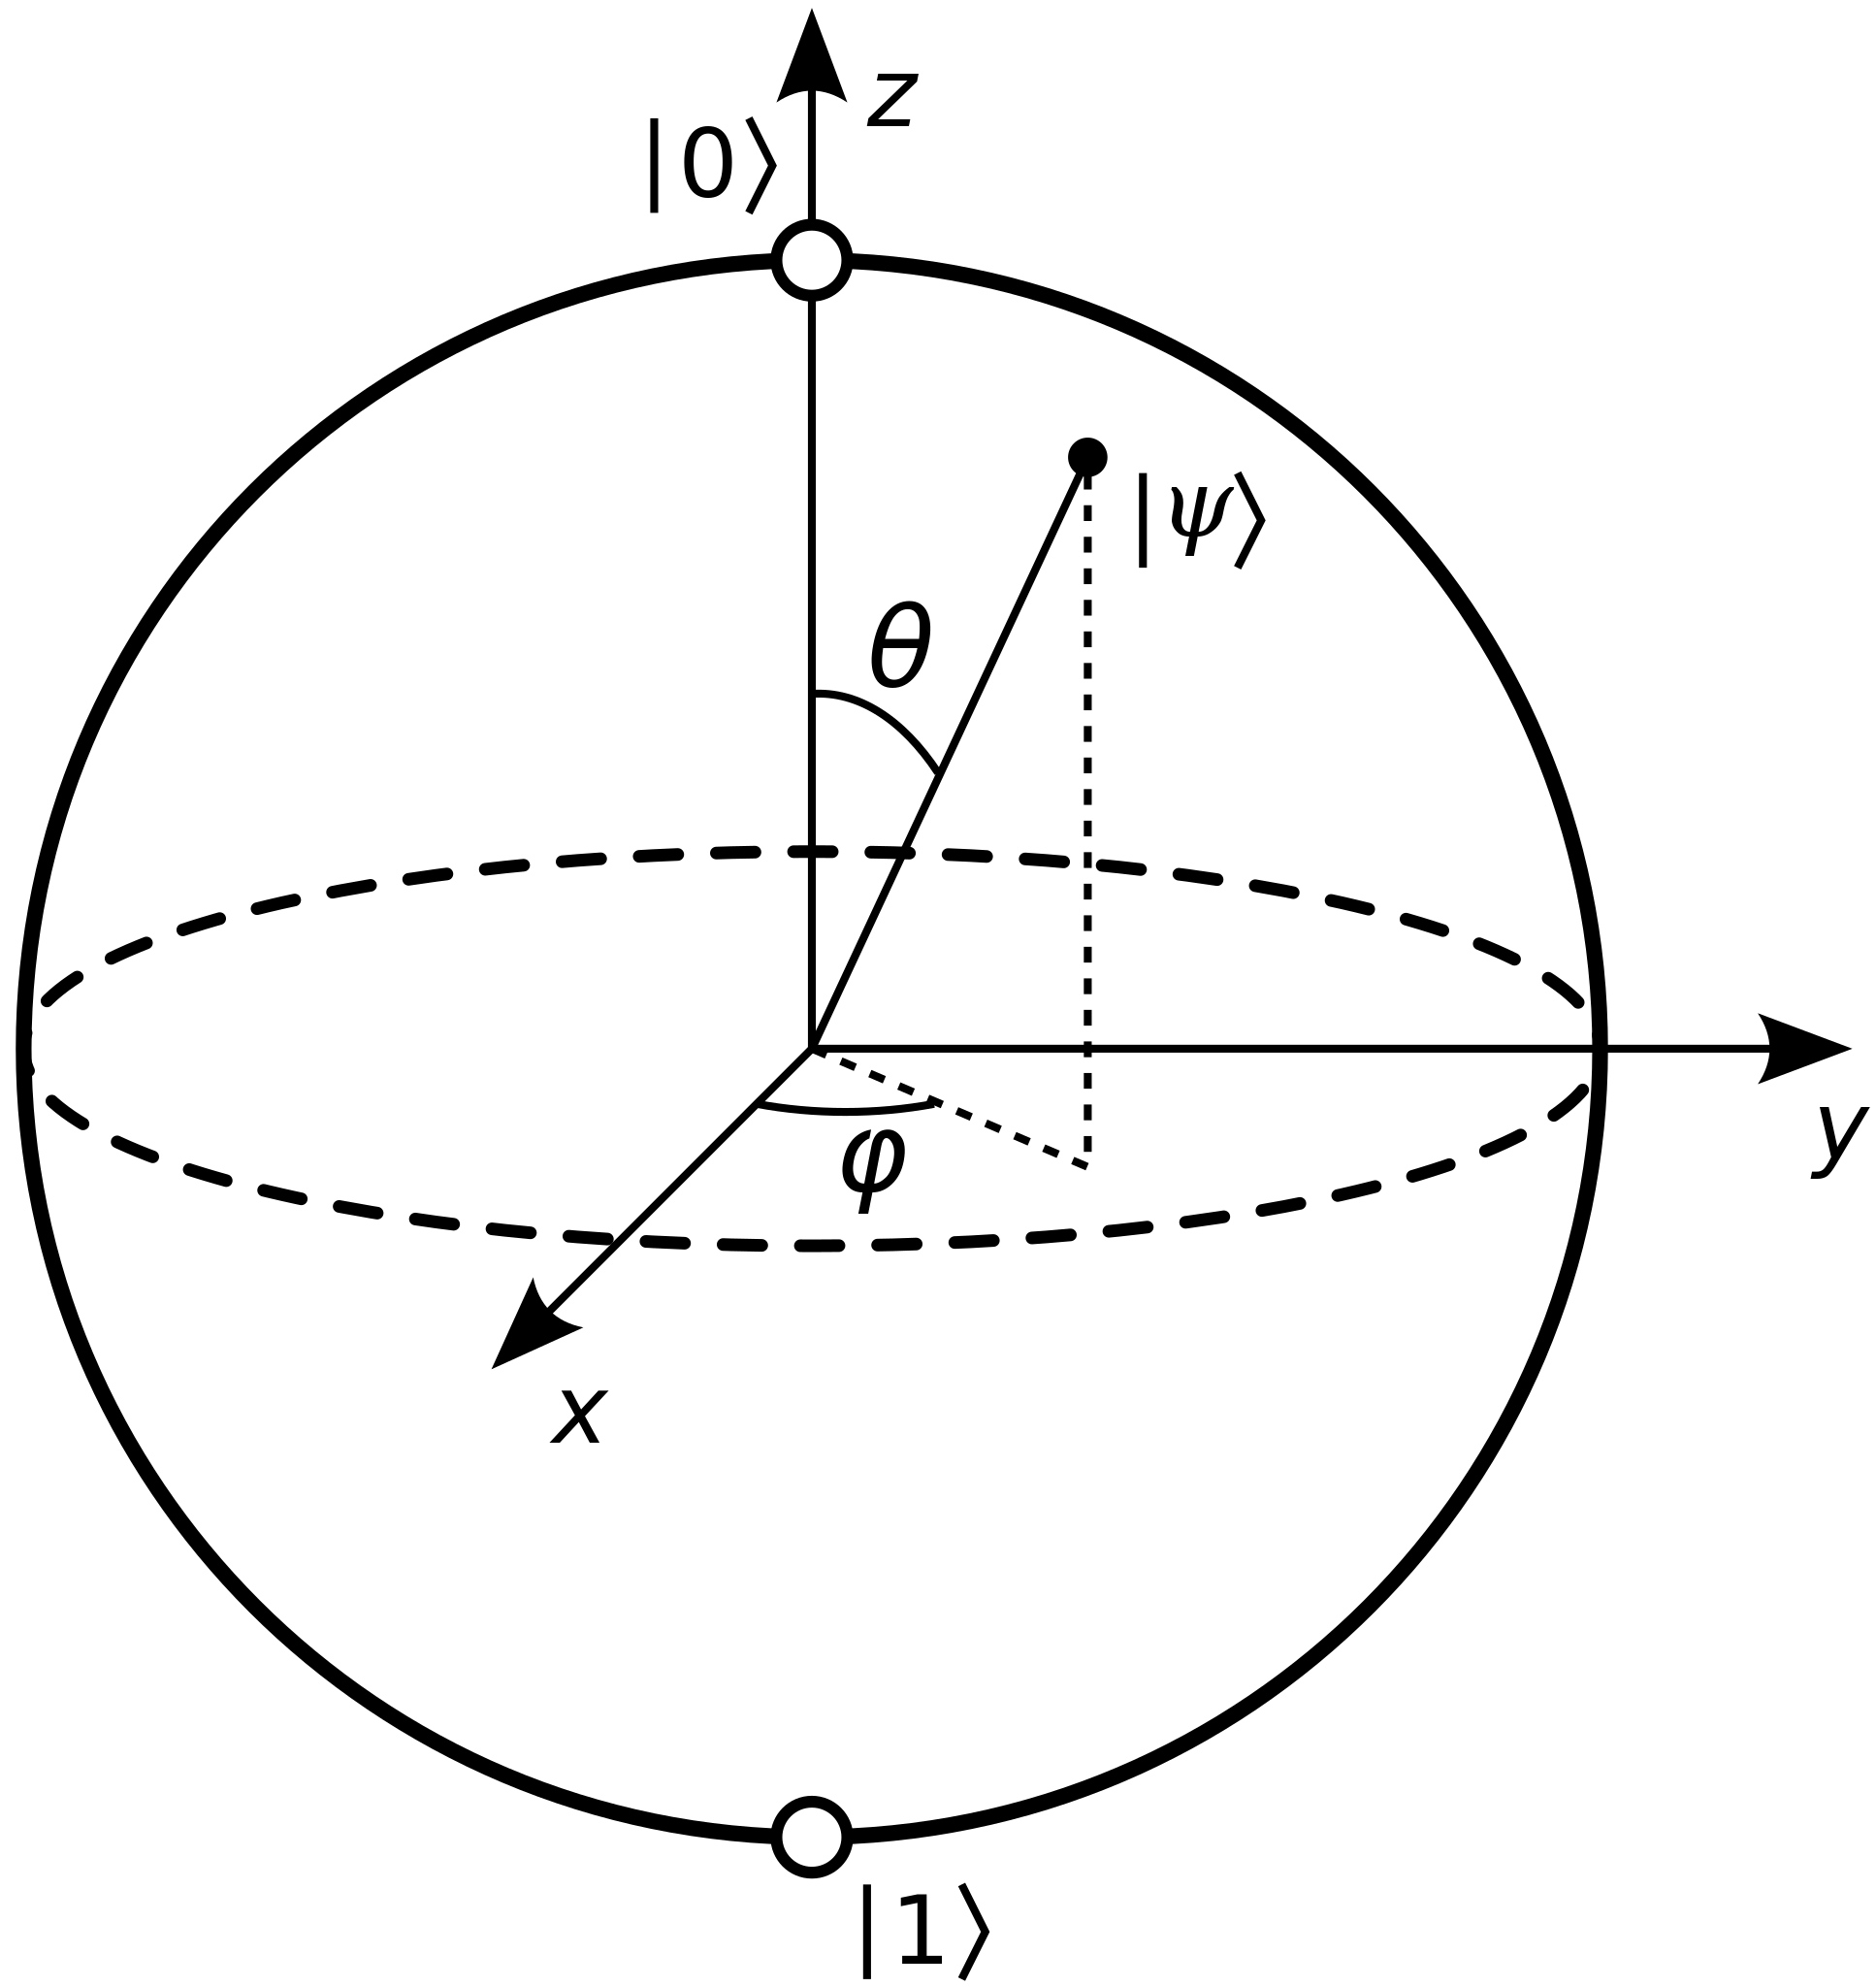
\includegraphics[scale=0.1]{figures/Bloch_sphere.png}
  \centering
  \caption{Bloch sphere representation of a qubit. Image taken from
           \href{https://commons.wikimedia.org/wiki/File:Bloch_Sphere.svg}{https://commons.wikimedia.org/wiki/File:Bloch\_Sphere.svg}
           under the \href{https://en.wikipedia.org/wiki/Creative_Commons}{Creative Commons Attribution-Share Alike 3.0 Unported license}.}
\end{figure}\label{fig:bloch_sphere} \

    - Introuce Bloch sphere \
    - Introduce many qubits system \
    - Introduce entanglement, 11 \ 
- Introduce quantum gates \
    - Equate a gate with a unitary matrix \
    - Pauli Gates \
    - Hadamard Gates \
- Introduce quantum circuits \
- Introduce quantum measurement \
\subsection{Density Operator}\label{subsection:density_operator}
- Introduce the density operator \
- Introduce quantum algorithms* \

i.	Introduce the required quantum concepts for the reader to understand noise in quantum computing.

\section{Quantum Noise}
i.	Describe the types of noise that can occur.
ii.	Explain where can noise occur.
iii.	State how noise can be simulated.

\section{Quantum Machine Learning}
i.	Present the difference between QML and classical ML\@.
ii.	Introduce variational quantum circuits.
iii.	Explain quantum kernel methods.

\section{Adversarial Machine Learning}
i.	State generalization problems.
ii.	Present different attacks such as FGSM, C\&W, and PGD\@.
iii.	Introduce adversarial training as defence mechanism against adversarial attacks.
iv.	Explain the relationship between general accuracy and adversarial resilience.